%% the main definitions for the report (KOMA-Script based)
\documentclass[11pt,a4paper]{scrreprt}
\usepackage[T1]{fontenc}
\usepackage[utf8]{inputenc}
\usepackage[german,english]{babel}
%\usepackage{layouts}
\usepackage{graphicx}

\begin{document}
\selectlanguage{\german}
\title{Benutzerhandbuch für WeatherInfo}
\author{SE3 Team}
\date{Juni 2009}

\maketitle

\tableofcontents

\chapter{Einleitung}
Das Programm WeatherInfo stellt Wetterinformationen, welche vom BBC-UK Weather Forecast
WebService geladen werden, graphisch dar und bietet dem Benutzer dabei verschiedene
Ansichten an.

\chapter{Die Benutzeroberfläche}
Die Benutzeroberfläche des Programmes basiert auf dem C++-Toolkit Qt, damit ist
es portabel und kann sowohl unter Linux, MacOSX und MS Windows ausgeführt werden.

\section{Das Hauptfenster}
Nach dem Starten des Programmes wird dem Benutzer das Hauptfenster angezeigt,
in welchem er zwischen den verschiedenen Ansichten wählen kann oder das
Programm beenden.

\begin{center}
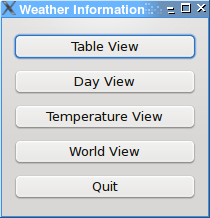
\includegraphics[width=7cm]{mainwidget.png}
\end{center}

\section{Die Tabellenansicht}
Die Tabellenansicht zeigt eine Übersicht aller verfügbaren Orte und das
Wetter an diesen innerhalb der nächsten 5 Tage.

\begin{center}
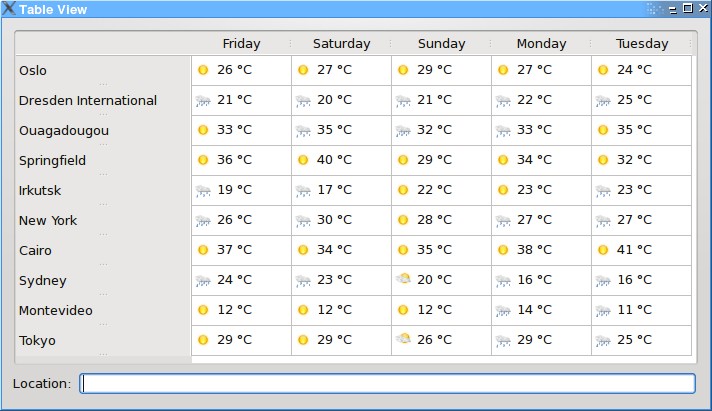
\includegraphics[width=14cm]{tableview.png}
\end{center}

Die Auswahl der angezeigten Orte kann vom Benutzer durch Eingabe eines
Namenfilters eingeschränkt werden.

\begin{center}
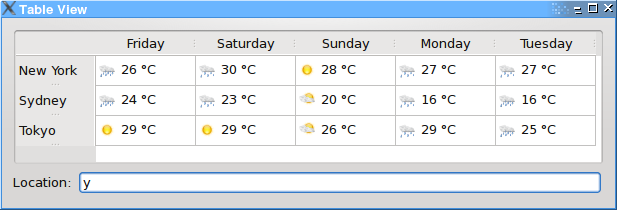
\includegraphics[width=14cm]{tableview_filtered.png}
\end{center}

Die Temperatur eines Ortes an einem Tag kann durch einen Doppelclick auf
die entsprechende Tabellenzelle und Eingabe des neuen Temperaturwertes
geändert werden.

\section{Die Ortsansicht}
Die Ortsansicht zeigt die Wetterinformationen für einen bestimmten Ort
und Tag an. Der Benutzer kann Ort und Tag selbst auswählen.

\begin{center}
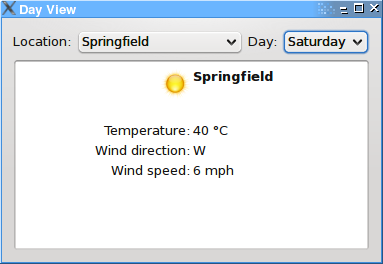
\includegraphics[width=14cm]{dayview.png}
\end{center}

\section{Die Temperaturansicht}
Die Temperaturansicht zeigt den Temperaturverlauf der nächsten 5 Tage
für einen bestimmten Ort an, welcher vom Benutzer selbst ausgewählt
werden kann.

\begin{center}
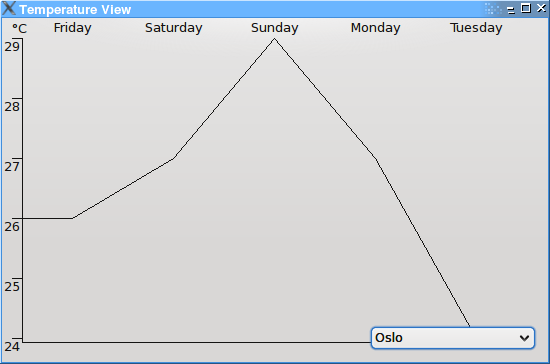
\includegraphics[width=14cm]{temperatureview.png}
\end{center}

\section{Die Weltansicht}
Die Weltansicht zeigt die Wetterbedingungen für einen bestimmten Tag
in allen verfügbaren Städten an. Der Benutzer kann den Tag selbst
auswählen.

\begin{center}
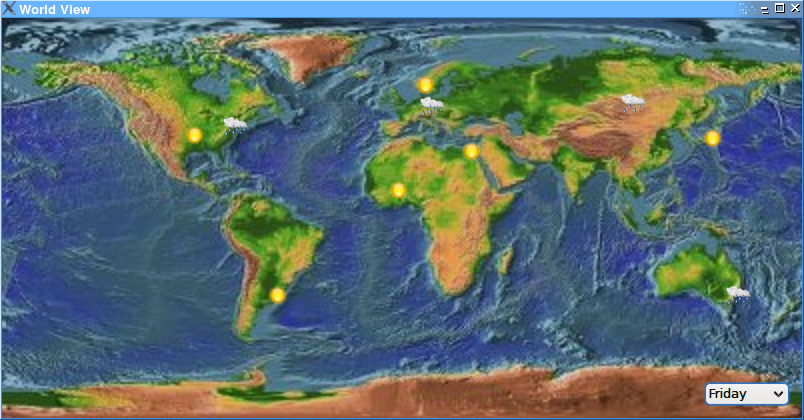
\includegraphics[width=14cm]{worldview.png}
\end{center}

\end{document}
